\part{Introduction}

\chapter{Description}

This plugin provides a shortcode\footnote{«Shortcodes are macros that can be
used to perform dynamic interactions with the content. i.e creating a gallery
from images attached to the post or rendering a video». \textsc{WordPress.org},
\textit{Plugin Handbook}, ``Shortcodes'',
\url{https://developer.wordpress.org/plugins/shortcodes/}.} to display a portion
of a post or page content only to users of a specific role. For example, you can
show the hidden text to Editors or to Authors or to any other WordPress role.
The plugin can also display the hidden text to specific users.

The action is performed using a shortcode, for example:

\begin{lstlisting}
[private role="administrator"]Text for administrators[/private]
\end{lstlisting}

In figure \vref{fig:shortcode-action} you can see an example of usage.

\begin{figure}[h]
	\centering
	\subfloat[][The webpage when the visitor doesn't have rights to read the
	hidden message. There is no text between the two paragraphs, even in the
	\textsc{html} source
	page.]{\fbox{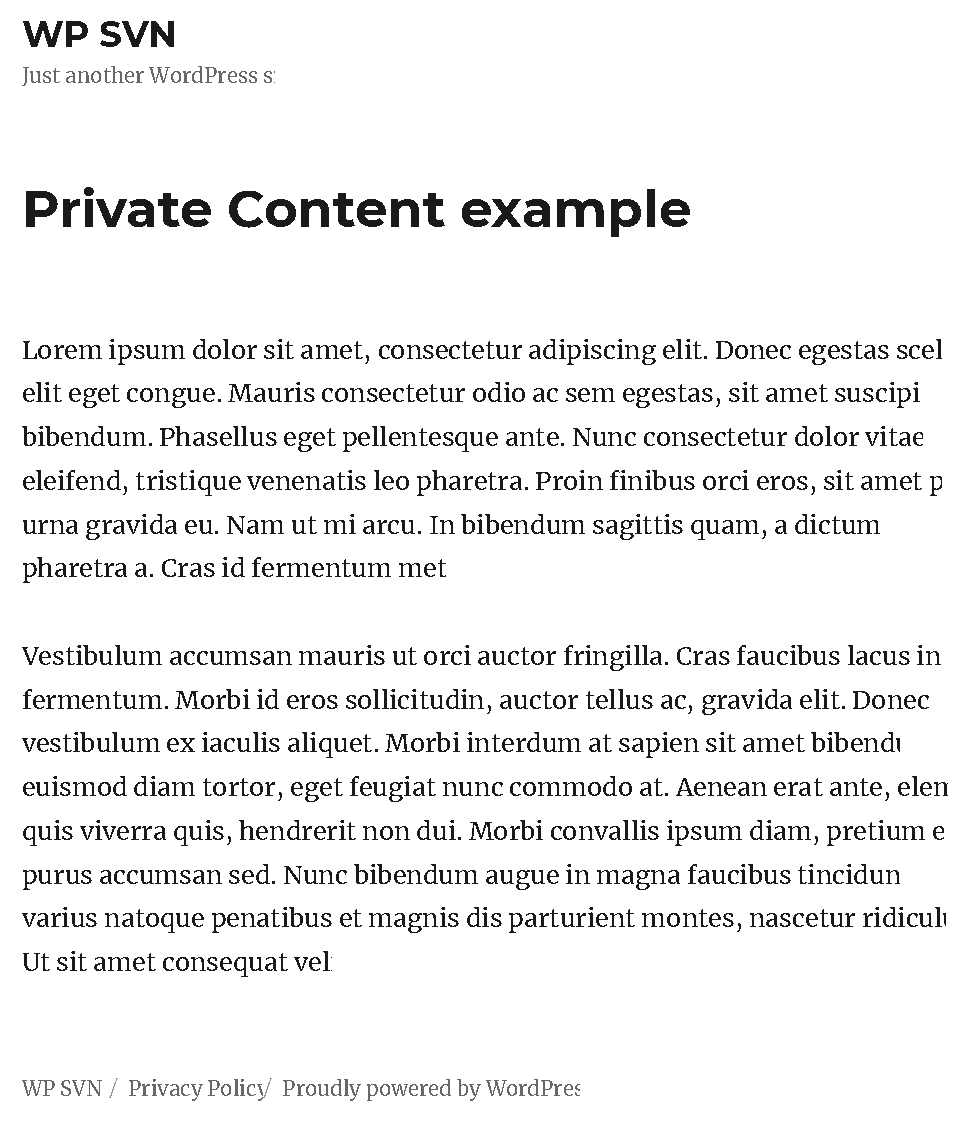
\includegraphics[width=.45\textwidth]{no-message.pdf}}} \quad
	\subfloat[][The webpage when the visitor has rights to read the hidden
	message. The green background has been added via
	\textsc{css}.]{\fbox{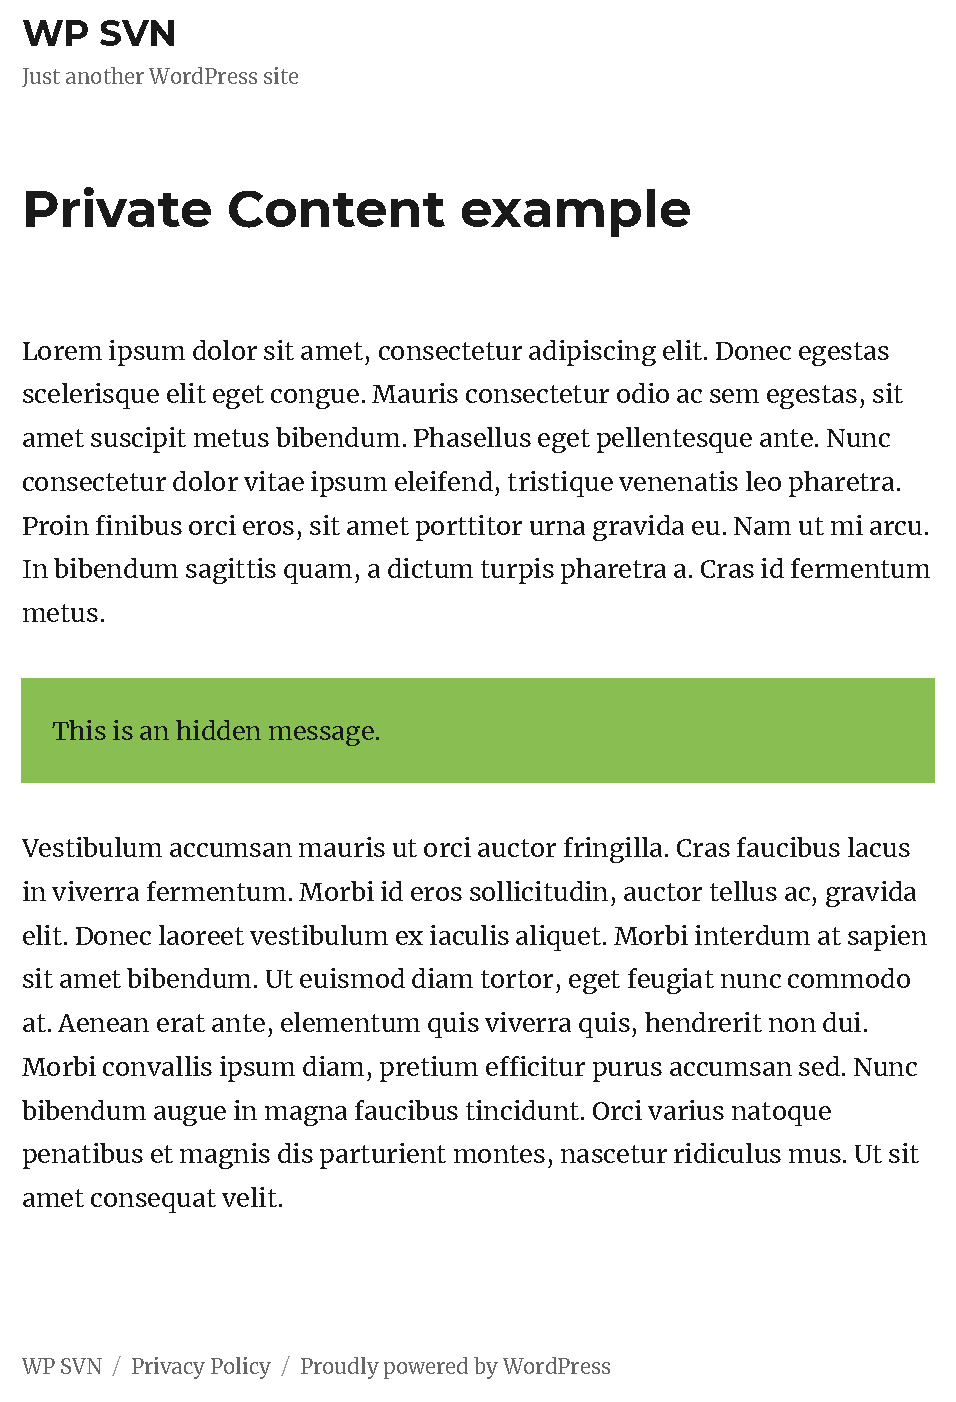
\includegraphics[width=.45\textwidth]{with-message.pdf}}}
	\caption{The shortcode in action.}
	\label{fig:shortcode-action}
\end{figure}

Please, note that an Administrator can read an Editor private content or a
Subscriber private content, and so on. Same thing for Editor, Author,
Contributor, and Subscriber: \textit{a higher role can read a lower role
content} (in almost all cases, see the paragraph \vref{multiple-custom-roles}
\textit{Multiple custom roles} for more information), according to the following
WordPress roles\footnote{For more information see \textsc{WordPress.org},
\textit{Plugin Handbook}, ``Roles and Capabilities'',
\url{https://wordpress.org/support/article/roles-and-capabilities/}.} schema in
descending order:

\begin{itemize}
	\item Administrator
	\item Editor
	\item Author
	\item Contributor
	\item Subscriber
\end{itemize}

Also you can show the hidden text \textit{only} to a certain role. For example,
you can mark a text as visible only to Contributors and hide it to higher roles,
such as Administrators or Editors and so on.

\part{The shortcode}

\chapter{The shortcode command}

The shortcode is \verb+[private]+:

\begin{lstlisting}
[private {attributes}]Text[/private]
\end{lstlisting}

There is another shortcode available \verb+[ubn_private]+, that can be used just
in case \verb+private+ is already taken by another plugin:

\begin{lstlisting}
[ubn_private {attributes}]Text[/ubn_private]
\end{lstlisting}

\chapter{The shortcode attributes}

These are the available attributes for the shortcode, that will be explained in
the next sections of this page:

\begin{itemize}
 \item \verb+role+
 \item \verb+recipient+
 \item \verb+custom_role+
 \item \verb+reverse+
 \item \verb+align+
 \item \verb+alt+
 \item \verb+container+
 \item \verb+id+
 \item \verb+class+
\end{itemize}

\section{\{role\} Text for a certain role}

Accepted arguments:

\begin{itemize}
 \item \verb+administrator+
 \item \verb+editor+
 \item \verb+editor-only+
 \item \verb+author+
 \item \verb+author-only+
 \item \verb+contributor+
 \item \verb+contributor-only+
 \item \verb+subscriber+
 \item \verb+subscriber-only+
 \item \verb+visitor+ or \verb+visitor-only+ (they are equivalent)
 \item \verb+none+
 \item \verb+custom+
 \item \verb+custom-only+
 \item \verb+post-author+
 \item \verb+post-author-only+
\end{itemize}

Let's see them in detail in the figure \vref{fig:role-option} and in the table \vref{table:roles}.

\begin{figure}[]
	\centering
  \fbox{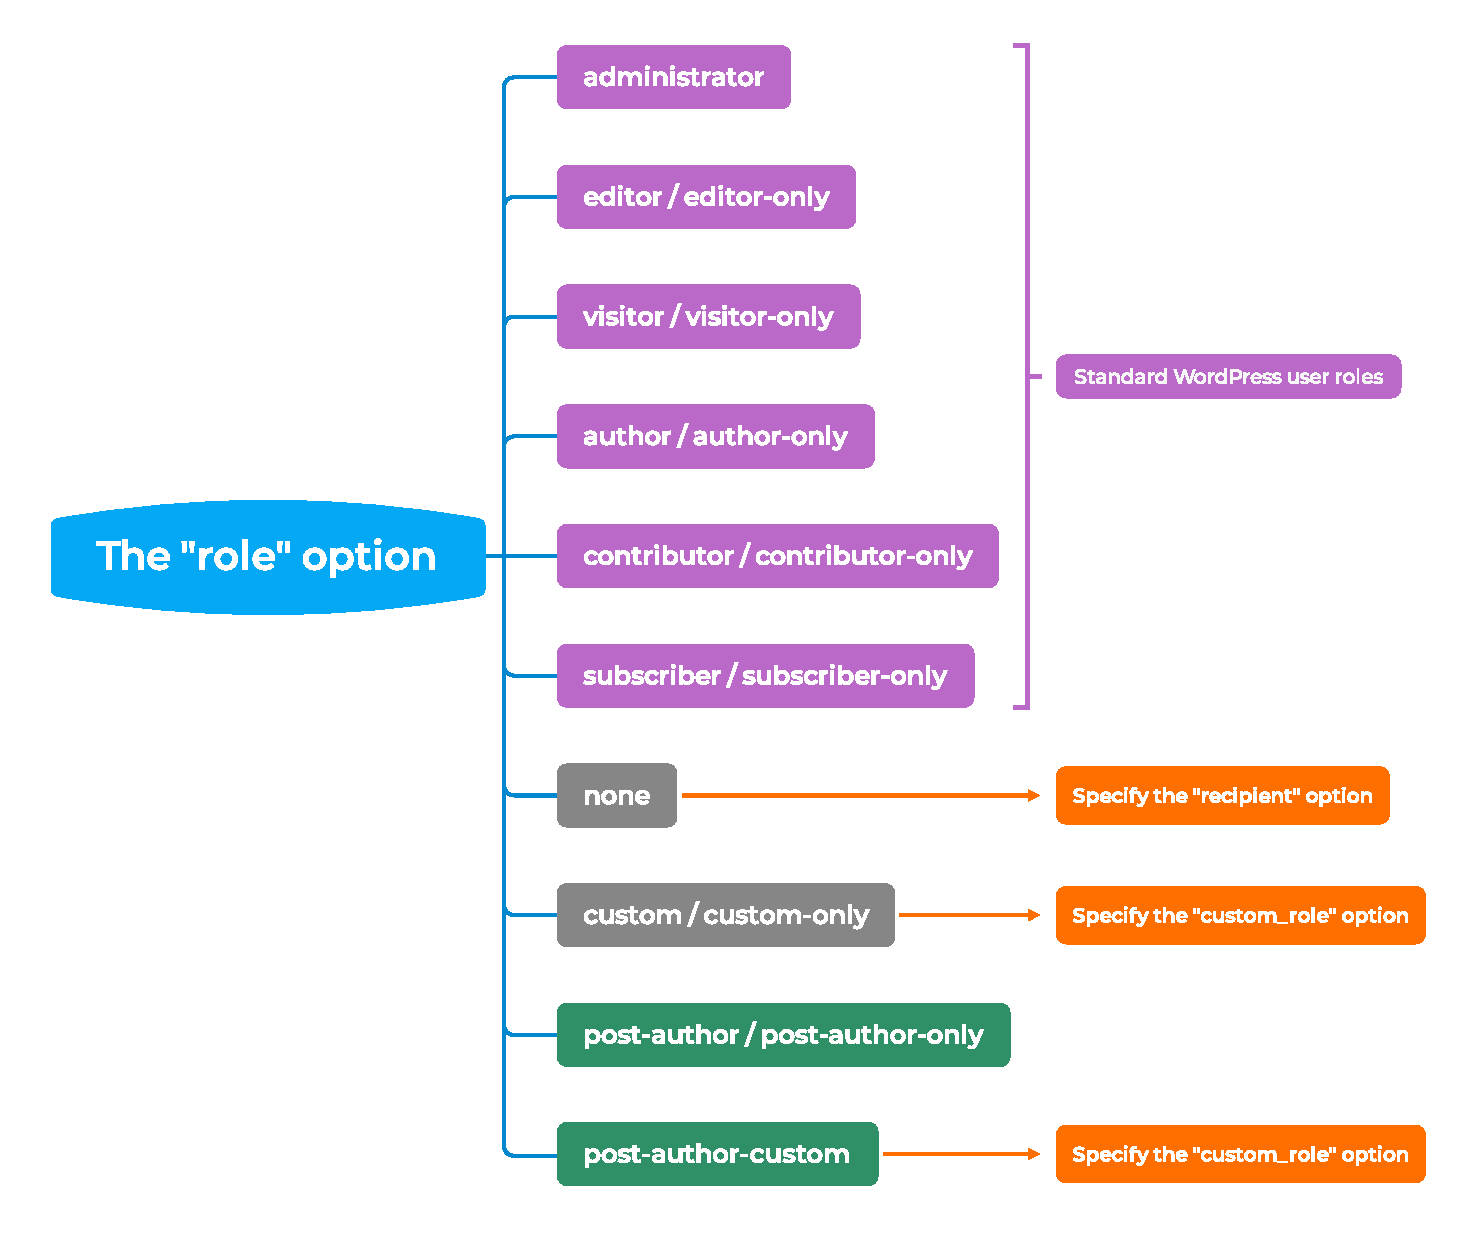
\includegraphics[width=1\textwidth]{role-option.pdf}}
	\caption{The \texttt{role} option.}
  \label{fig:role-option}
\end{figure}

\begin{table}
 \centering
 \begin{tabular}[t]{l p{7cm}}
 \toprule
 \textsc{Role} & \textsc{Result} \\
 \midrule
 \verb+administrator+ & The hidden text is shown to Administrators. \\
 \verb+editor+ & The hidden text is shown to Editors and Administrators. \\
 \verb+editor-only+ & The hidden text is shown to Editors only. \\
 \verb+author+ & The hidden text is shown to Authors, Editors, and
 Administrators. \\
 \verb+author-only+ & The hidden text is shown to Authors only. \\
 \verb+contributor+ & The hidden text is shown to Contributors, Authors,
 Editors, and Administrators. \\
 \verb+contributor-only+ & The hidden text is shown to Contributors only. \\
 \verb+subscriber+ & The hidden text is shown to Subscribers, Contributors,
 Authors, Editors, and Administrators. \\
 \verb+subscriber-only+ & The hidden text is shown to Subscribers only. \\
 \verb+visitor+ / \verb+visitor-only+ & The hidden text is shown only to
 non-logged-in users. \textit{Administrators can read the hidden text.} \\
 \verb+none+ & When used, it is mandatory to use also the \verb+recipient+
 option. The hidden text is shown only to users in the \verb+recipient+ list.
 \textit{Administrators cannot read the hidden text.} \\
 \verb+custom+ & When used, it is mandatory to use also the \verb+custom_role+
 option. The hidden text is shown only to users that have a role in the
 \verb+custom_role+ list. \textit{Administrators can read the hidden text.} \\
 \verb+custom-only+ & When used, it is mandatory to use also the
 \verb+custom_role+ option. The hidden text is shown only to users that have a
 role in the \verb+custom_role+ list. \textit{Administrators cannot read the
 hidden text.} \\
 \verb+post-author+ & The hidden text is shown to the author of the post.
 \textit{Administrators can read the hidden text.} \\
 \verb+post-author-only+ & The hidden text is shown to the author of the post
 only. \textit{Administrators cannot read the hidden text.} \\
 \bottomrule
 \end{tabular}
 \caption{Who can read the private text when a given role is used.}
 \label{table:roles}
\end{table}

\subsection{Examples}

Display the private text to Administrators:

\begin{lstlisting}
[private role="administrator"]Text for Administrators[/private]
\end{lstlisting}

Display the private text to Administrators and Editors:

\begin{lstlisting}
[private role="editor"]Text for Editors[/private]
\end{lstlisting}

Display the private text to Administrators, Editors, and Authors:

\begin{lstlisting}
[private role="author"]Text for Authors[/private]
\end{lstlisting}

Display the private text to Administrators, Editors, Authors, and Contributors:

\begin{lstlisting}
[private role="contributor"]Text for Contributor[/private]
\end{lstlisting}

Display the private text to Administrators, Editors, Authors, Contributors, and
Subscribers:

\begin{lstlisting}
[private role="subscriber"]Text for Subscribers[/private]
\end{lstlisting}

Display this text to the author of the current post:

\begin{lstlisting}
[private role="post-author"]Text for author of the post[/private]
\end{lstlisting}

\subsection{Text for specific roles excluding other roles}

If you want to show a note only to a certain role, you have to use a
\verb+{role}-only+ option. In this way, for example, an Administrator or an
Editor (roles higher than Author) cannot read a note for Authors only. These are
all the cases:

Display the private text to Editors only:

\begin{lstlisting}
[private role="editor-only"]Text for Editors only[/private]
\end{lstlisting}

Display the private text to Authors only:

\begin{lstlisting}
[private role="author-only"]Text for Authors only[/private]
\end{lstlisting}

Display the private text to Contributors only:

\begin{lstlisting}
[private role="contributor-only"]Text for Contributors only[/private]
\end{lstlisting}

Display the private text to Subscribers only:

\begin{lstlisting}
[private role="subscriber-only"]Text for Subscribers only[/private]
\end{lstlisting}

Display the private text to Visitors only:

\begin{lstlisting}
[private role="visitor-only"]Text for Visitors only[/private]
\end{lstlisting}

or the equivalent shortcode:

\begin{lstlisting}
[private role="visitor"]Text for Visitors only[/private]
\end{lstlisting}

Display this text to the author of the current post only:

\begin{lstlisting}
[private role="post-author-only"]Text for author of the post only[/private]
\end{lstlisting}

Display the private text to Designers only (Designers is a custom role created
by the user):

\begin{lstlisting}
[private role="custom-only" custom_role="designers"]Text for Designers only[/private]
\end{lstlisting}

\section{\{recipient\} Text for a specific or multiple users}

Accepted arguments:

\begin{itemize}
  \item login name of the target user. You can use multiple login names, comma
  separated;
  \item user \textsc{id}\footnote{By default, WordPress hides the \textsc{id}s
  of elements like posts, pages, users, and so on. To display these \textsc{id}s
  and use them in the shortcode you can install a dedicated plugin, like
  \textit{Reveal IDs} by Oliver Schlöbe, available at
  \url{https://wordpress.org/plugins/reveal-ids-for-wp-admin-25/}.} of the
  target user. You can use multiple user \textsc{id}s, comma separated;
  \item login names and user \textsc{id}s mixed together.
\end{itemize}

In the case you want to show a text only to a specific user, assign \verb+none+
to \verb+role+ and a login name to \verb+recipient+:

\begin{lstlisting}
[private role="none" recipient="login-name"]Text for a specific user only[/private]
\end{lstlisting}

Change \verb+login-name+ with the correct login name of the target user.

You can use a comma separated list of usernames to target certain users:

\begin{lstlisting}
[private role="none" recipient="login-name1, login-name2, login-name3"]Text for specific users only[/private]
\end{lstlisting}

Change \verb+login-name1+, \verb+login-name2+, and \verb+login-name3+ with the
correct login names of the target users.

Also, you can use user \textsc{id}s to target users, for example:

\begin{lstlisting}
  [private role="none" recipient="5, 31, 27"]Text for specific users only[/private]
\end{lstlisting}

\section{\{custom\_role\} Text for custom or multiple roles}

Accepted arguments:

\begin{itemize}
 \item the custom role
 \item the custom roles, comma separated
\end{itemize}

\subsection{Single custom role}

If you want to show a text only to users of a custom role, use the option
\verb+custom_role+.

For example:

\begin{lstlisting}
[private role="custom" custom_role="designers"]Text for Designers group.[/private]
\end{lstlisting}


Please, note that texts for custom roles can be read also by Administrators. To
avoid this, use the \verb+role="custom-only"+ option, followed by the name of
the custom role.

For example:

\begin{lstlisting}
[private role="custom-only" custom_role="designers"]Text for Designers only.[/private]
\end{lstlisting}

The option \verb+role=custom+ can be used also for the WordPress standard roles,
for example:

\begin{lstlisting}
[private role="custom" custom_role="author"]Text for role Author.[/private]
\end{lstlisting}

In this case, Authors will read the private text, but higher roles (such as
Editors) will not read it. It is like using a \verb+role-only+ option. Anyway,
Administrators will read it. For more information, see the paragraph
\vref{multiple-custom-roles} \textit{Multiple custom roles}.

\subsection{Multiple custom roles}\label{multiple-custom-roles}

If you want to show a text to multiple roles, you can enter them separated by a
comma. For example:

\begin{lstlisting}
[private role="custom" custom_role="designers,engineers"]Text for Designers and Engineers groups.[/private]
\end{lstlisting}

You can mix custom roles and standard WordPress roles, with a \textit{caveat}
explained in the paragraph \vref{caveat}.

For example:

\begin{lstlisting}
[private role="custom" custom_role="designers,engineers,author"]Text for Designers, Engineers, and Authors group.[/private]
\end{lstlisting}

As you can see, Designers and Engineers are custom roles, while Author is a
standard WordPress role. In the above example, Administrator will read the
private text. Even in this case, as wrote before, you can use the
\verb+role="custom-only"+ option to prevent Administrators from reading the
private text:

\begin{lstlisting}
[private role="custom-only" custom_role="designers,engineers,author"]Text for Designers, Engineers, and Authors group.[/private]
\end{lstlisting}

\subsection{Caveat}\label{caveat}

A note on using standard WordPress \graffito{A note when using WordPress
standard roles here.} roles with the option \verb+role=custom+. If you use a
standard WordPress role with the \verb+custom_role+ option, you expect that a
higher role can read the private text for lowers roles, i.e. a text for the
Author role should be read by the Editor role (which is a role higher that
Author). Actually, the Editor role won't read that text. This is normal, because
the option \verb+role="custom"+ follows a path different than standard WordPress
role management. It's like you'd use a \verb+role-only+ option, in our example a
\verb+role="author-only"+ option. For example, this shortcode:

\begin{lstlisting}
[private role="custom" custom_role="designers,engineers,author"]Text for Designers, Engineers, and Authors group.[/private]
\end{lstlisting}

\noindent will be read by Designers, Engineers, Authors, and Administrators, but
not by Editors (even if Editor is a higher role than Author).

\section{\{reverse\} Reverse the logic of hiding text}

Accepted arguments:

\begin{itemize}
 \item \verb+1+ --- Activate the reverse option
\end{itemize}

The option \verb+reverse=1+ is used when you want to hide a private text to some
users or to some custom roles. Since it would be uncomfortable to add a lot of
users/group in the shortcode, it is more convenient to tell the plugin to show
the private text to all users/groups and hide it to some.

The \verb+reverse+ option is available only with the following options:

\begin{itemize}
 \item \textit{single users:} \verb+role=none+, adding also the \verb+recipient+ option
 and the \verb+reverse+;
 \item \textit{custom roles:} \verb+role=custom+, adding also the \verb+custom_role+
 option and the \verb+reverse+.
\end{itemize}

See here below the two cases.

\subsection{Use of the \{reverse\} option for single users}

If you want to show a text to all users but not to some, activate the option
\verb+reverse+, so that users added in the \verb+recipient+ option will not read
the note.

For example:

\begin{lstlisting}
[private role="none" recipient="alice,bob,charlie" reverse=1]We all read this message while Alice, Bob, and Charlie can't read it![/private]
\end{lstlisting}

This shortcode will show the text to all users, excluding Alice, Bob, and
Charlie (which cannot read the text).

\subsection{Use of the \{reverse\} option for roles}

You can use the \verb+reverse+ option also when using roles. In this case you
will not use the \verb+recipient+ option, but simply in this way:

\begin{lstlisting}
[private role="custom" custom_role="designers" reverse=1]Text for all roles, excluding Designers.[/private]
\end{lstlisting}

With this shortcode, all users will read the private message, while Designers
will be excluded. If you define an alternate message with \verb+alt+ option,
Designers will read the alternate message only.

You can also exclude multiple roles. For example:

\begin{lstlisting}
[private role="custom" custom_role="designers, engineers, author" reverse=1 alt="You can't read hidden texts because you are part of Designers and/or Engineers and/or Author roles"]Text for all roles, excluding Designers, Engineers, and Author roles.[/private]
\end{lstlisting}

Take note that Administrators will read the hidden text, even if the current
Administrator has also one or more of the excluded roles. See the section
\vref{sec:admin-role} for more information and also the table \vref{table:roles}.

\section{\{align\} Align style}

Accepted arguments:

\begin{itemize}
 \item \verb+left+ --- Left align the paragraph
 \item \verb+center+ --- Center align the paragraph
 \item \verb+right+ --- Right align the paragraph
 \item \verb+justify+ --- Justify the paragraph
\end{itemize}

\section{\{alt\} Alternate text for excluded users}

If you want to show an alternate text in case the reader can't read the hidden
text, you can use:

\begin{lstlisting}
[private role="author" alt="You have not rights to read this."]Text for authors only[/private]
\end{lstlisting}

Please, take note that, if defined, the alternate text is always publicly
displayed to users without the rights to read the hidden text.

The alternate text can contain some \textsc{html} tags. The list is:

\begin{itemize}
 \item \verb+b+ or \verb+strong+ for bold text;
 \item \verb+em+ or \verb+i+ for italic text;
 \item \verb+a+ for links, with \verb+href+ and \verb+title+ included. For
 \verb+href+ and \verb+title+ do not use double quote, but single quote.
\end{itemize}

For example:

\begin{lstlisting}
[private role="subscriber" alt="<a href='https://www.example.com/subscribe' title='Subscribe now!'>Subscribe</a> to read this <strong>super powered</strong> text!"]Hidden text.[/private]
\end{lstlisting}

\section{\{container\} The \textsc{html} container for the text}

Starting from version 2.4, the user can choose the \textsc{html} container
element for the text.

Accepted arguments:

\begin{itemize}
 \item \verb+p+ --- The default value;
 \item \verb+div+ --- This element allows you use \textsc{html} elements like
 lists, headings, and more.
 \item \verb+span+ --- This element allows you to add private content inline.
\end{itemize}

Examples:

Wrap the note inside a \textsc{div}:

\begin{lstlisting}
[private container="div"]This is the text[/private]
\end{lstlisting}

Wrap the note inside a \textsc{span}:

\begin{lstlisting}
This is my home I bought a year ago [private container="span"](the key is under the doormat)[/private].
\end{lstlisting}


\section{\{id\} Custom \textsc{id}s for the \textsc{html} container}

The user of the plugin can add custom \textsc{id}s to the \textsc{html}
container using the option \verb+id="name-of-the-id"+, for example:

\begin{lstlisting}
[private id="myid1, custom-id-2, my_id_3"]Private text.[/private]
\end{lstlisting}

The single \textsc{id} names should be separated by a comma. Also, if the
\textsc{id} is composed by more words, the words must be separated by a dash or
by an underscore, otherwise the single words will be considered as separated
\textsc{id} names.

\section{\{class\} Custom classes for the \textsc{html} container}

The user of the plugin can add custom classes to the \textsc{html} container
using the option \verb+class="name-of-the-class"+, for example:

\begin{lstlisting}
[private class="myclass1, custom-class-2, my_class_3"]Private text.[/private]
\end{lstlisting}

The single class names should be separated by a comma. Also, if the class is
composed by more words, the words must be separated by a dash or by an
underscore, otherwise the single words will be considered as separated class
names. Only consider that underscores will be changed into a dash, starting from
version 6.4.0.

\chapter{The Administrator role}

\label{sec:admin-role}

The Administrator role is a special role in this plugin. This role can always
read the hidden texts, unless one of these options has been used:

\begin{itemize}
 \item a \verb+{role}-only+ option (excluding \verb+visitor+ and
 \verb+visitor-only+);
 \item a \verb+none+ (with \verb+recipient+) option;
 \item a \verb+custom-only+ option.
\end{itemize}

For example, let's say that the role Designers has been excluded from reading a
hidden text. If an Administrator is reading that page and he has also the
Designers role, he will read the hidden text. In the following example,
Administrator (which has the Designer role too) can read the hidden text:

\begin{lstlisting}
[private role="custom" custom_role="designers" reverse=1]Text for all roles, excluding Designers role.[/private]
\end{lstlisting}

In the following examples, instead, Administrators cannot read the hidden texts:

\begin{lstlisting}
[private role="author-only"]Private note for Author.[/private]
\end{lstlisting}

\begin{lstlisting}
[private role="post-author-only"]Private note for the author of the post.[/private]
\end{lstlisting}

\begin{lstlisting}
[private role="none" recipient="john"]Private note for John.[/private]
\end{lstlisting}

\begin{lstlisting}
[private role="custom-only" custom_role="engineers"]Private note for Engineers role.[/private]
\end{lstlisting}

\chapter{Nesting shortcodes}

With Private Content you can nest a shortcode inside another shortcode. For
example, you have a paragraph dedicated to Author and Marketing roles, but a
portion of that text should be displayed to Marketing role only. For this
purpose, you can nest a shortcode inside another.

Only take note that you can't use the same shortcode name for both the outer
shortcode and the nested shortcode: this is due to how WordPress handles the
shortcode names.\footnote{For more information see \textsc{WordPress.org},
\textit{Shortcode API}, ``Nested shortcodes'',
\url{https://codex.wordpress.org/Shortcode_API\#Nested_Shortcodes}.}
In other words, you can't do this:

\begin{lstlisting}
  [private]Text
    [private]Nested text.[/private]
    Text.
  [/private]
\end{lstlisting}

Having in mind that Private Content has two names available,\footnote{Private
Content has two shortcode names available since version 4.3. The new name was
introduced in the case the name \texttt{private} was taken by another plugin.}
\texttt{[private]} and \texttt{[ubn\_private]}, the correct nesting would be:

\begin{lstlisting}
  [private]Text
    [ubn_private]Nested text.[/ubn_private]
    Text.
  [/private]
\end{lstlisting}

In our example, a nested shortcode could be:

\begin{lstlisting}
  [private role="custom" custom_role="author, marketing" container="div"]Leading text for Author and Marketing.
  [ubn_private role="custom" custom_role="marketing"]Text for Marketing only.[/ubn_private]
  Trailing text for Author and Marketing.[/private]
\end{lstlisting}

When nesting shortcodes, \graffito{Use \texttt{div} as container when nesting
shortcodes.} it is advisable to use the \textsc{div} tag as container, because
the standard P tag may produce unexpected results (for example, empty P tags
and/or text without an \textsc{html} tag).

\part{Style \& testing}

\chapter{Giving a style to the private text}

The text generated by this plugin uses some \textsc{css} classes, listed here:

\begin{itemize}
 \item \verb+private+ --- Applied to each \textsc{html} element generated by this
 plugin.
 \item \verb+{role}-content+ --- Applied to the text for a particular role. Here
 is the complete list:
 \begin{itemize}
  \item \verb+administrator-content+
  \item \verb+editor-content+
  \item \verb+author-content+
  \item \verb+contributor-content+
  \item \verb+subscriber-content+
  \item \verb+visitor-content+
  \item \verb+user-content+ --- When used for specific user(s).
  \begin{itemize}
   \item \verb+user-only+ --- When used for specific user(s). This class is
   always preceded by \verb+user-content+ class.
    \item \verb+{user_login}-only+ --- When used for specific user(s). The
    placeholder \verb+{user_login}+ will be changed into the actual login name.
    This class is always preceded by \verb+user-content+ and \verb+user-only+
    classes.
    \item \verb+user-only-reverse+ --- When the \verb+reverse+ option is used.
    This class is always preceded by \verb+user-content+ class.
  \end{itemize}
  \item \verb+{custom_role}-content+ --- When used for custom roles. The
  placeholder \verb+{custom_role}+ will be changed into the actual custom role.
  \end{itemize}
 \item \verb+{role}-only+ --- Applied to the text for a specific role. This
 class is always preceded by \verb+{role}-content+ class.
 \item \verb+{custom-id-names}+ --- Added when specified by the user.
 \item \verb+{custom-class-names}+ --- Added when specified by the user.
 \item \verb+alt-text+ --- Applied to the alternate text.
\end{itemize}

\chapter{Testing the shortcode}

It could be useful to test if the shortcode is working as intended. To do this,
you can use a plugin that lets you temporarily switch between accounts. The
plugin is \textit{User Switching} by John Blackbourn \& contributors, available
at:
\begin{center}
  \url{https://wordpress.org/plugins/user-switching}
\end{center}

After having inserted the shortcode in the post/page, switch to the user account
in the user management page using the relevant link, then visit the published
page. You should see the page as the user will see it.

\part{Developer notes}

\chapter{Capabilities created by Private Content}

These are the capabilities created by this plugin:

\begin{itemize}
 \item \verb+read_ubn_editor_notes+
 \item \verb+read_ubn_author_notes+
 \item \verb+read_ubn_contributor_notes+
 \item \verb+read_ubn_subscriber_notes+
\end{itemize}

These capabilities will be removed when the plugin is uninstalled using the
usual uninstallation command in the WordPress Dashboard.

\chapter{Available filters}

\begin{itemize}
 \item \verb+ubn_private_align_style+ --- Filters the style string. An example of
 a string is:
\end{itemize}

\begin{lstlisting}
$align_style = ' style="text-align: justify;"';
\end{lstlisting}

Please note the leading space before \verb+style=+.

\begin{itemize}
 \item \verb+ubn_private_containers+ --- Filters the array containing the
 \textsc{html} container for the private and alternate text.
\end{itemize}

An example is:

\begin{lstlisting}
$containers = array(
  'open'  => '<p',
  'close' => '</p>',
);
\end{lstlisting}

Notice that the first element of the array must not have the closing \verb+>+.

\begin{itemize}
 \item \verb+ubn_private_content+ --- Filters the private content.
 \item \verb+ubn_private_alt+ --- Filters the alternate content.
 \item \verb+ubn_private_text+ --- Filters the entire private and alternate text,
 just before the output. The string contains also the \textsc{html} container.
 \item \verb+ubn_private_text_empty+ --- Filters the text if it is empty, just
 before the output.
 \item \verb+ubn_private_class_selector+ --- Filters the \textsc{html} output for
 the classes.
 \item \verb+ubn_private_id_selector+ --- Filters the \textsc{html} output for the
 \textsc{id}s.
\end{itemize}



\chapter{Uninstallation}

The plugin can be simply uninstalled from the WordPress Dashboard. During the
uninstallation process, the plugin removes its files and the modifications
created during the installation. The removed modifications are:

\begin{itemize}
  \item remove \texttt{read\_ubn\_editor\_notes} capability from the Editor role;
  \item remove \texttt{read\_ubn\_author\_notes} capability from the Author role;
  \item remove \texttt{read\_ubn\_contributor\_notes} capability from the Contributor role;
  \item remove \texttt{read\_ubn\_subscriber\_notes} capability from the Subscriber role.
\end{itemize}

\vfill

\begin{figure}[h]
	\centering
	
\includegraphics[width=.6\textwidth]{noah-boyer-dgBOx1e3Mbs-unsplash}
  \caption{\emph{So long, and thanks for all the fish.}\\(\textsc{Douglas Adams})}
	\label{fig:dolphin}
\end{figure}
